\documentclass{standalone}
\usepackage{tikz}
\usetikzlibrary{patterns, positioning}


\begin{document}
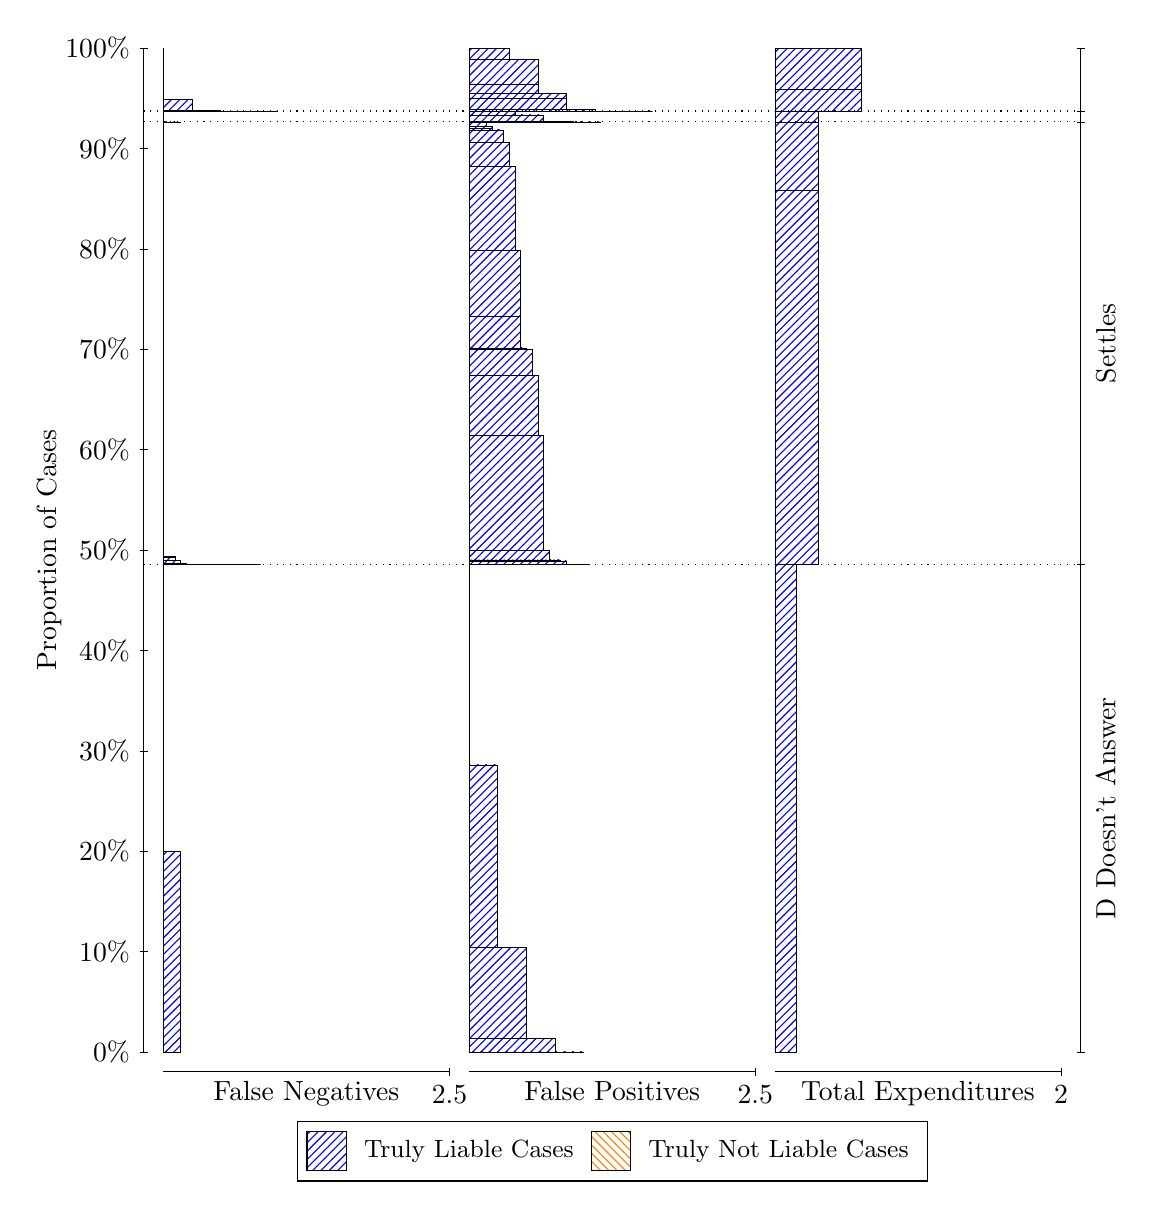
\begin{tikzpicture}
\draw[black, very thin] (1.5,1.75) -- (1.5,14.5);
\node[rotate=90, text=black, anchor=center] at (0.3, 8.125) {Proportion of Cases};
\draw[black, very thin] (1.45,1.75) -- (1.55,1.75);
\node[text=black, anchor=east] at (1.45, 1.75) {0\%};
\draw[black, very thin] (1.45,3.025) -- (1.55,3.025);
\node[text=black, anchor=east] at (1.45, 3.025) {10\%};
\draw[black, very thin] (1.45,4.3) -- (1.55,4.3);
\node[text=black, anchor=east] at (1.45, 4.3) {20\%};
\draw[black, very thin] (1.45,5.575) -- (1.55,5.575);
\node[text=black, anchor=east] at (1.45, 5.575) {30\%};
\draw[black, very thin] (1.45,6.85) -- (1.55,6.85);
\node[text=black, anchor=east] at (1.45, 6.85) {40\%};
\draw[black, very thin] (1.45,8.125) -- (1.55,8.125);
\node[text=black, anchor=east] at (1.45, 8.125) {50\%};
\draw[black, very thin] (1.45,9.4) -- (1.55,9.4);
\node[text=black, anchor=east] at (1.45, 9.4) {60\%};
\draw[black, very thin] (1.45,10.675) -- (1.55,10.675);
\node[text=black, anchor=east] at (1.45, 10.675) {70\%};
\draw[black, very thin] (1.45,11.95) -- (1.55,11.95);
\node[text=black, anchor=east] at (1.45, 11.95) {80\%};
\draw[black, very thin] (1.45,13.225) -- (1.55,13.225);
\node[text=black, anchor=east] at (1.45, 13.225) {90\%};
\draw[black, very thin] (1.45,14.5) -- (1.55,14.5);
\node[text=black, anchor=east] at (1.45, 14.5) {100\%};

\draw[black, very thin] (13.4,1.75) -- (13.4,14.5);
\draw[black, very thin] (13.35,1.75) -- (13.45,1.75);
\node[anchor=west] at (13.35, 1.75) {};
\draw[black, very thin] (13.35,7.9424) -- (13.45,7.9424);
\node[anchor=west] at (13.35, 7.9424) {};
\draw[black, very thin] (13.35,13.562) -- (13.45,13.562);
\node[anchor=west] at (13.35, 13.562) {};
\draw[black, very thin] (13.35,13.7) -- (13.45,13.7);
\node[anchor=west] at (13.35, 13.7) {};
\draw[black, very thin] (13.35,14.5) -- (13.45,14.5);
\node[anchor=west] at (13.35, 14.5) {};

\draw[black, very thin, pattern color=blue, pattern=north east lines] (1.75,1.75) rectangle (1.968,4.2976);
\draw[black, very thin, pattern color=orange, pattern=north west lines] (1.75,4.2976) rectangle (1.75,4.2976);
\draw[black, very thin, pattern color=blue, pattern=north east lines] (1.75,4.2976) rectangle (1.75,7.9424);
\draw[black, very thin, pattern color=blue, pattern=north east lines] (1.75,7.9424) rectangle (2.9853,7.9424);
\draw[black, very thin, pattern color=blue, pattern=north east lines] (1.75,7.9424) rectangle (2.6947,7.9424);
\draw[black, very thin, pattern color=blue, pattern=north east lines] (1.75,7.9424) rectangle (2.622,7.9424);
\draw[black, very thin, pattern color=blue, pattern=north east lines] (1.75,7.9424) rectangle (2.5493,7.9424);
\draw[black, very thin, pattern color=blue, pattern=north east lines] (1.75,7.9424) rectangle (2.404,7.9424);
\draw[black, very thin, pattern color=blue, pattern=north east lines] (1.75,7.9424) rectangle (2.3313,7.9425);
\draw[black, very thin, pattern color=blue, pattern=north east lines] (1.75,7.9425) rectangle (2.2587,7.9425);
\draw[black, very thin, pattern color=blue, pattern=north east lines] (1.75,7.9425) rectangle (2.186,7.9425);
\draw[black, very thin, pattern color=blue, pattern=north east lines] (1.75,7.9425) rectangle (2.1133,7.9443);
\draw[black, very thin, pattern color=blue, pattern=north east lines] (1.75,7.9443) rectangle (2.0407,7.951);
\draw[black, very thin, pattern color=blue, pattern=north east lines] (1.75,7.951) rectangle (1.968,7.9961);
\draw[black, very thin, pattern color=blue, pattern=north east lines] (1.75,7.9961) rectangle (1.8953,8.0277);
\draw[black, very thin, pattern color=blue, pattern=north east lines] (1.75,8.0277) rectangle (1.8953,8.044);
\draw[black, very thin, pattern color=blue, pattern=north east lines] (1.75,8.044) rectangle (1.8227,8.0448);
\draw[black, very thin, pattern color=orange, pattern=north west lines] (1.75,8.0448) rectangle (1.75,8.0448);
\draw[black, very thin, pattern color=blue, pattern=north east lines] (1.75,8.0448) rectangle (1.75,13.562);
\draw[black, very thin, pattern color=blue, pattern=north east lines] (1.75,13.562) rectangle (1.968,13.563);
\draw[black, very thin, pattern color=orange, pattern=north west lines] (1.75,13.563) rectangle (1.75,13.563);
\draw[black, very thin, pattern color=blue, pattern=north east lines] (1.75,13.563) rectangle (1.75,13.7);
\draw[black, very thin, pattern color=blue, pattern=north east lines] (1.75,13.7) rectangle (3.2033,13.7);
\draw[black, very thin, pattern color=blue, pattern=north east lines] (1.75,13.7) rectangle (2.84,13.7);
\draw[black, very thin, pattern color=blue, pattern=north east lines] (1.75,13.7) rectangle (2.4767,13.705);
\draw[black, very thin, pattern color=blue, pattern=north east lines] (1.75,13.705) rectangle (2.1133,13.846);
\draw[black, very thin, pattern color=orange, pattern=north west lines] (1.75,13.846) rectangle (1.75,13.846);
\draw[black, very thin, pattern color=blue, pattern=north east lines] (1.75,13.846) rectangle (1.75,14.5);
\draw[black, very thin, pattern color=orange, pattern=north west lines] (5.6333,1.75) rectangle (7.0867,1.75);
\draw[black, very thin, pattern color=blue, pattern=north east lines] (5.6333,1.75) rectangle (7.0867,1.7518);
\draw[black, very thin, pattern color=blue, pattern=north east lines] (5.6333,1.7518) rectangle (6.7233,1.9273);
\draw[black, very thin, pattern color=blue, pattern=north east lines] (5.6333,1.9273) rectangle (6.36,3.0778);
\draw[black, very thin, pattern color=blue, pattern=north east lines] (5.6333,3.0778) rectangle (5.9967,5.3949);
\draw[black, very thin, pattern color=blue, pattern=north east lines] (5.6333,5.3949) rectangle (5.6333,7.9424);
\draw[black, very thin, pattern color=orange, pattern=north west lines] (5.6333,7.9424) rectangle (7.1593,7.9424);
\draw[black, very thin, pattern color=blue, pattern=north east lines] (5.6333,7.9424) rectangle (7.1593,7.9424);
\draw[black, very thin, pattern color=orange, pattern=north west lines] (5.6333,7.9424) rectangle (7.014,7.9424);
\draw[black, very thin, pattern color=blue, pattern=north east lines] (5.6333,7.9424) rectangle (7.014,7.9427);
\draw[black, very thin, pattern color=orange, pattern=north west lines] (5.6333,7.9427) rectangle (6.8687,7.9427);
\draw[black, very thin, pattern color=blue, pattern=north east lines] (5.6333,7.9427) rectangle (6.8687,7.988);
\draw[black, very thin, pattern color=blue, pattern=north east lines] (5.6333,7.988) rectangle (6.796,7.9993);
\draw[black, very thin, pattern color=orange, pattern=north west lines] (5.6333,7.9993) rectangle (6.7233,7.9993);
\draw[black, very thin, pattern color=blue, pattern=north east lines] (5.6333,7.9993) rectangle (6.7233,8.0005);
\draw[black, very thin, pattern color=blue, pattern=north east lines] (5.6333,8.0005) rectangle (6.6507,8.1166);
\draw[black, very thin, pattern color=orange, pattern=north west lines] (5.6333,8.1166) rectangle (6.578,8.1166);
\draw[black, very thin, pattern color=blue, pattern=north east lines] (5.6333,8.1166) rectangle (6.578,9.5815);
\draw[black, very thin, pattern color=blue, pattern=north east lines] (5.6333,9.5815) rectangle (6.5053,10.341);
\draw[black, very thin, pattern color=blue, pattern=north east lines] (5.6333,10.341) rectangle (6.4327,10.669);
\draw[black, very thin, pattern color=blue, pattern=north east lines] (5.6333,10.669) rectangle (6.36,10.692);
\draw[black, very thin, pattern color=blue, pattern=north east lines] (5.6333,10.692) rectangle (6.2873,11.094);
\draw[black, very thin, pattern color=orange, pattern=north west lines] (5.6333,11.094) rectangle (6.2873,11.094);
\draw[black, very thin, pattern color=blue, pattern=north east lines] (5.6333,11.094) rectangle (6.2873,11.934);
\draw[black, very thin, pattern color=blue, pattern=north east lines] (5.6333,11.934) rectangle (6.2147,12.997);
\draw[black, very thin, pattern color=blue, pattern=north east lines] (5.6333,12.997) rectangle (6.142,13.302);
\draw[black, very thin, pattern color=blue, pattern=north east lines] (5.6333,13.302) rectangle (6.0693,13.46);
\draw[black, very thin, pattern color=blue, pattern=north east lines] (5.6333,13.46) rectangle (5.9967,13.461);
\draw[black, very thin, pattern color=blue, pattern=north east lines] (5.6333,13.461) rectangle (5.924,13.477);
\draw[black, very thin, pattern color=blue, pattern=north east lines] (5.6333,13.477) rectangle (5.924,13.509);
\draw[black, very thin, pattern color=blue, pattern=north east lines] (5.6333,13.509) rectangle (5.8513,13.554);
\draw[black, very thin, pattern color=blue, pattern=north east lines] (5.6333,13.554) rectangle (5.7787,13.56);
\draw[black, very thin, pattern color=blue, pattern=north east lines] (5.6333,13.56) rectangle (5.706,13.562);
\draw[black, very thin, pattern color=blue, pattern=north east lines] (5.6333,13.562) rectangle (5.6333,13.562);
\draw[black, very thin, pattern color=orange, pattern=north west lines] (5.6333,13.562) rectangle (7.3047,13.562);
\draw[black, very thin, pattern color=blue, pattern=north east lines] (5.6333,13.562) rectangle (7.3047,13.562);
\draw[black, very thin, pattern color=blue, pattern=north east lines] (5.6333,13.562) rectangle (6.9413,13.565);
\draw[black, very thin, pattern color=blue, pattern=north east lines] (5.6333,13.565) rectangle (6.578,13.651);
\draw[black, very thin, pattern color=blue, pattern=north east lines] (5.6333,13.651) rectangle (6.2147,13.7);
\draw[black, very thin, pattern color=blue, pattern=north east lines] (5.6333,13.7) rectangle (5.8513,13.7);
\draw[black, very thin, pattern color=orange, pattern=north west lines] (5.6333,13.7) rectangle (7.9587,13.7);
\draw[black, very thin, pattern color=blue, pattern=north east lines] (5.6333,13.7) rectangle (7.9587,13.7);
\draw[black, very thin, pattern color=orange, pattern=north west lines] (5.6333,13.7) rectangle (7.5953,13.7);
\draw[black, very thin, pattern color=blue, pattern=north east lines] (5.6333,13.7) rectangle (7.5953,13.7);
\draw[black, very thin, pattern color=orange, pattern=north west lines] (5.6333,13.7) rectangle (7.232,13.7);
\draw[black, very thin, pattern color=blue, pattern=north east lines] (5.6333,13.7) rectangle (7.232,13.72);
\draw[black, very thin, pattern color=blue, pattern=north east lines] (5.6333,13.72) rectangle (6.8687,13.86);
\draw[black, very thin, pattern color=orange, pattern=north west lines] (5.6333,13.86) rectangle (6.8687,13.86);
\draw[black, very thin, pattern color=blue, pattern=north east lines] (5.6333,13.86) rectangle (6.8687,13.921);
\draw[black, very thin, pattern color=blue, pattern=north east lines] (5.6333,13.921) rectangle (6.5053,14.038);
\draw[black, very thin, pattern color=orange, pattern=north west lines] (5.6333,14.038) rectangle (6.5053,14.038);
\draw[black, very thin, pattern color=blue, pattern=north east lines] (5.6333,14.038) rectangle (6.5053,14.354);
\draw[black, very thin, pattern color=blue, pattern=north east lines] (5.6333,14.354) rectangle (6.142,14.355);
\draw[black, very thin, pattern color=blue, pattern=north east lines] (5.6333,14.355) rectangle (6.142,14.495);
\draw[black, very thin, pattern color=blue, pattern=north east lines] (5.6333,14.495) rectangle (5.7787,14.495);
\draw[black, very thin, pattern color=blue, pattern=north east lines] (5.6333,14.495) rectangle (5.7787,14.5);
\draw[black, very thin, pattern color=blue, pattern=north east lines] (5.6333,14.5) rectangle (5.6333,14.5);
\draw[black, very thin, pattern color=orange, pattern=north west lines] (9.5167,1.75) rectangle (9.7892,1.75);
\draw[black, very thin, pattern color=blue, pattern=north east lines] (9.5167,1.75) rectangle (9.7892,7.9424);
\draw[black, very thin, pattern color=orange, pattern=north west lines] (9.5167,7.9424) rectangle (10.062,7.9424);
\draw[black, very thin, pattern color=blue, pattern=north east lines] (9.5167,7.9424) rectangle (10.062,12.691);
\draw[black, very thin, pattern color=orange, pattern=north west lines] (9.5167,12.691) rectangle (10.062,12.691);
\draw[black, very thin, pattern color=blue, pattern=north east lines] (9.5167,12.691) rectangle (10.062,13.562);
\draw[black, very thin, pattern color=orange, pattern=north west lines] (9.5167,13.562) rectangle (10.062,13.562);
\draw[black, very thin, pattern color=blue, pattern=north east lines] (9.5167,13.562) rectangle (10.062,13.7);
\draw[black, very thin, pattern color=orange, pattern=north west lines] (9.5167,13.7) rectangle (10.607,13.7);
\draw[black, very thin, pattern color=blue, pattern=north east lines] (9.5167,13.7) rectangle (10.607,13.978);
\draw[black, very thin, pattern color=orange, pattern=north west lines] (9.5167,13.978) rectangle (10.607,13.978);
\draw[black, very thin, pattern color=blue, pattern=north east lines] (9.5167,13.978) rectangle (10.607,14.5);
\draw[black, dotted] (1.5,7.9424) -- (13.4,7.9424);
\draw[black, dotted] (1.5,13.562) -- (13.4,13.562);
\draw[black, dotted] (1.5,13.7) -- (13.4,13.7);
\draw[black, very thin] (1.75,1.5) -- (5.3833,1.5);
\node[text=black, anchor=north] at (3.5667, 1.5) {False Negatives};
\draw[black, very thin] (5.3833,1.45) -- (5.3833,1.55);
\node[text=black, anchor=north] at (5.3833, 1.45) {2.5};

\draw[black, very thin] (5.6333,1.5) -- (9.2667,1.5);
\node[text=black, anchor=north] at (7.45, 1.5) {False Positives};
\draw[black, very thin] (9.2667,1.45) -- (9.2667,1.55);
\node[text=black, anchor=north] at (9.2667, 1.45) {2.5};

\draw[black, very thin] (9.5167,1.5) -- (13.15,1.5);
\node[text=black, anchor=north] at (11.333, 1.5) {Total Expenditures};
\draw[black, very thin] (13.15,1.45) -- (13.15,1.55);
\node[text=black, anchor=north] at (13.15, 1.45) {2};

\node[text=black, centered, rotate=90] at (13.72, 4.8462) {D Doesn't Answer};
\node[text=black, centered, rotate=90] at (13.72, 10.752) {Settles};



\draw (7.449999999999999,1.5) node[draw=none] (baseCoordinate) {};
\begin{scope}[align=center]
        \matrix[scale=0.5, draw=black, below=0.5cm of baseCoordinate, nodes={draw}, column sep=0.1cm]{
            \node[rectangle, draw, minimum width=0.5cm, minimum height=0.5cm, pattern color=blue, pattern=north east lines] {}; &
            \node[draw=none, font=\small, text=black] (B) {Truly Liable Cases}; &
            \node[rectangle, draw, minimum width=0.5cm, minimum height=0.5cm, pattern color=orange, pattern=north west lines] {}; &
            \node[draw=none, font=\small, text=black] (B) {Truly Not Liable Cases}; \\
            };
\end{scope}

\end{tikzpicture}
\end{document}